\documentclass[show notes]{beamer}
% \usepackage{graphicx} % Required for inserting images
%\usepackage{lipsum}
\usepackage{multicol}
\usepackage{dcolumn}
\usepackage{blindtext}
\usepackage{minitoc}

\usetheme{Marburg}
\usecolortheme{albatross}

\title{Quantencomputing}
\subtitle{CS1025 Hauptseminar}
\author{Nils Jannik Schulze-Clewing}
\institute{THM}
\date{June 2024}

% Neuer Befehl für Sections mit kurzen und langen Titeln
\newcommand{\mysection}[3][]{
    \section[#1]{#2}
    \begin{frame}{#2}
        #3
        \label{frame:#2}
    \end{frame}
}

% Neuer Befehl für Subsections mit kurzen und langen Titeln
\newcommand{\mysubsection}[3][]{
    \subsection[#1]{#2}
    \begin{frame}{#2}
        #3
        \label{frame:#2}
    \end{frame}
}
\newcommand{\mysubsubsection}[2]{
    \subsubsection{#1}
    \begin{frame}{#1}
    #2
        \label{frame:#1}
    \end{frame}
}

\begin{document}

\begin{frame}{\titlepage}
    
\end{frame}

\begin{frame}{Handout}
QR-Code

Link
\end{frame}

\begin{frame}{Übersicht}
    \tableofcontents
\end{frame}

\mysection[Motivation]{Motivation und Perspektiven}{

}

\note{
Impact ähnlich KI

Wenige Jahre

Eigene Fazination
}


\mysection[Quantenphänomene]{Phänomene der Quantenwelt}{
    \begin{itemize}
        \item Doppelspalt
        \item Spukhafte Fernwirkung
    \end{itemize}
}


\mysubsection[Doppelsplalt]{Doppelspalt Experiment}{
    
    \only<1>{
    \begin{figure}
        \centering
        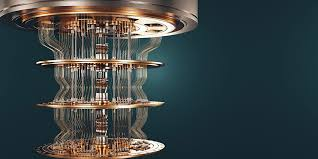
\includegraphics[width=0.5\linewidth]{img/Testbild.jpeg}
        \caption{Enter Caption}
        \label{fig:enter-label}
    \end{figure}
    }

    \only<2>{
    Echter Zufall
    Bild mit Münze einfügen
    }

    \only<3>{
    Konsequenz
    }
}
\mysubsection[Spukhafte Fernwirkung]{Spukhafte Fernwirkung}{

    \only<1>{
    Einschub Photonen Messung
    }
    \only<2>{
    Bild vom gespaltenen Laiser
    }

    \only<3>{
    informationsgehalt immer identisch
    }
}

\mysection[Grundlagen]{Grundlagen Quantencomputing}{

}

\mysubsection[Photonen]{Eigenschaften von Photonen}{
    
}

\mysubsection[Qbits]{Bits und Qbits}{

}

\mysection[Quantenschaltkreise]{Quantenschaltkreise}{

}

\mysubsection[Pauli-X]{Pauli-X}{

}

\mysubsection[Pauli-Z]{Pauli-Z}{

}

\mysubsection[Hadamard]{Hadamard}{

}

\mysubsection[CNOT]{CNOT}{

}

\mysection[Teleportation]{Teleportation}{

}


\mysection[Quellen]{Quellen}{

}
\end{document}
